\chapter{Overview of the Compiler}

\section[17.1 Components of the Compiler]{17.1 Components of the Compiler}

The Icon compiler is divided into two components: a run-time system
and the compiler itself. This organization is illustrated below. In
the diagram, labeled boxes represent programs, other text (some of it
delimited by braces) represents files, and arrows represent data flow.

%-%\noindent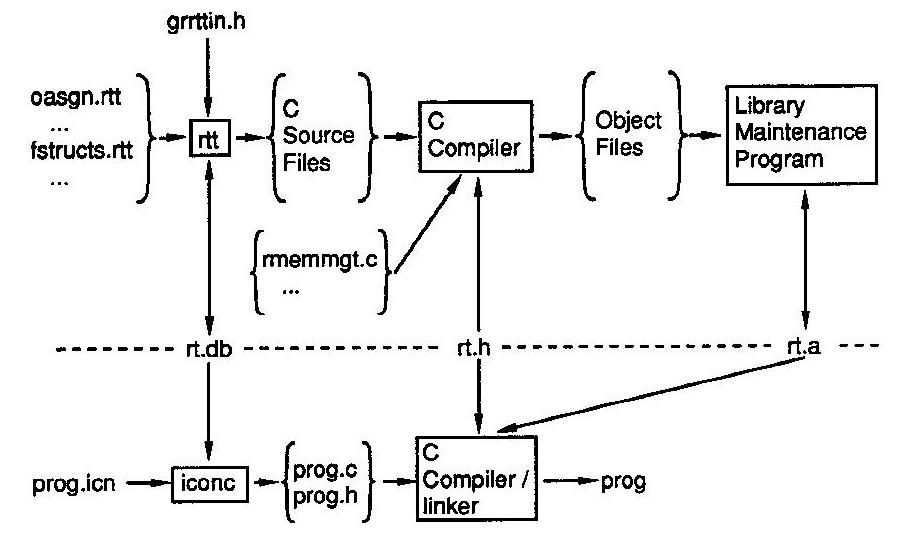
\includegraphics[width=6.0in,height=3.3in]{kw/figure5-1.png}

\begin{figure}[htb]
\noindent
\begin{tikzpicture}[very thick, >=latex, arrows=->,
    box/.style={rectangle, minimum width=10mm, draw},
    txt/.style={align=left, inner sep=0.5em},
    tbox/.style={rectangle,draw,align=left},
  ]
\matrix[row sep=0.4cm, column sep=0.7cm]{
% Row 1
  & \node(gth) {grttin.h}; &  &  &  & &[-0.7cm]  \\
% Row 2
\node(rttf)[txt]{oasgn.rtt\\~~\ldots\\fstructs.rtt\\~~\ldots};
  & \node(rtt)[box] {rtt};
  & \node(csf)[txt] {C\\Source\\Files};
  & \node(cc) [tbox]{C\\Compiler};
  & \node(of) [txt] {Object\\Files};
  & \node(lmp)[tbox]{Library\\Maintenance\\Program};\\
% Row 3
  &  & \node(rmc)[txt] {rmemmgt.c\\~~\ldots};   &  &  &  \\
% Row 4
\node(ds){};  & \node(rtdb) {rt.db}; &  & \node(rth) {rt.h};  &  & \node(rta) {rt.a}; & \node(de){};\\[1cm]
% Row 5
\node(picn) {prog.icn};
  & \node(iconc)[box]{iconc};
  & \node(pch)[txt]{prog.c\\prog.h};
  & \node(ccl)[tbox]{C\\Compiler /\\Linker};
  & \node(prog){prog};& \\
};
\draw (gth) -- (rtt); \draw[<->] (rtt) -- (rtdb); \draw (rtdb) -- (iconc);
\draw[dashed,arrows=-] (ds.west) -- (rtdb) -- (rth) -- (rta) -- (de.east)[xshift=1cm];
\draw[<->] (lmp) -- (rta);
\draw (rth) -- (cc); \draw (rth) -- (ccl);
\draw (rmc.east) -- (cc);
\draw (rta) -- ($(ccl.north) + (0.2,0.05)$);


\draw[-,decorate,decoration=brace] ($(rttf.north east)-(0.15,0)$) -- ($(rttf.south east)-(0.15,0)$);
\foreach \n in {csf, rmc, pch, of} {
  \draw[-,decorate,decoration=brace] ($(\n.south west)+(0.15,0)$) -- ($(\n.north west)+(0.15,0)$);
  \draw[-,decorate,decoration=brace] ($(\n.north east)-(0.15,0)$) -- ($(\n.south east)-(0.15,0)$);
};
\draw (rttf.east) -- (rtt); \draw (rtt) -- (csf.west);
\draw (csf.east) -- (cc);   \draw (cc) -- (of.west); \draw (of.east) -- (lmp);

\draw (picn) -- (iconc);   \draw (iconc) -- (pch.west);
\draw (pch.east) -- (ccl); \draw (ccl) -- (prog);
\end{tikzpicture}
\caption{Organization of the compiler and run-time system}
\end{figure}

The run-time system appears above the dotted line and the compiler
itself appears below the line. The programs shown with the run-time
system are executed once when the run-time system is installed or
updated. They build a data base, rt.db, and an object-code library,
rt.a, for use by the compiler. The general definition of the term
{\textasciigrave}{\textasciigrave}data base'{}' is used here: a
collection of related data. rt.db is stored as a text file. It is
accessed and manipulated in internal tables by the programs rtt and
iconc. The rtt program is specific to the Icon compiler system and is
described below. The C compiler and the library maintenance program
are those native to the system on which the Icon compiler is being
used. The format of the object-code library is dictated by the linker
used with the C compiler. The file rt.h contains C definitions shared
by the routines in the run-time system and code generated by the
compiler.

The diagram of the compiler itself reflects the fact that the Icon
compiler uses a C compiler and linker as a back end.  However, iconc
automatically invokes these programs, so the Icon programmer sees a
single tool that takes Icon source as input and produces an executable
file.


\section[17.2 The Run-time System]{17.2 The Run-time System}

As with the run-time system for the interpreter, the run-time system
for the compiler implements Icon's operations.  However, the compiler
has needs beyond those of the interpreter. In the interpreter's
run-time system, all operations are implemented as C functions
conforming to certain conventions. The interpreter uses the same
implementation of an operation for all uses of the operation. While
this approach results in acceptable performance for many Icon
programs, the purpose of an optimizing compiler is to obtain better
performance. A major goal in the development of iconc is to use
information from type inferencing to tailor the parameter passing and
parameter type conversions of an operation to particular uses of the
operation and to place code in line where appropriate. The compiler
needs a mechanism to support this tailored operation invocation. In
addition, the compiler needs information about the properties of
operations for use in performing type inferencing and other analyses.

In addition to supporting the analyses and optimizations of iconc,
there are several other major goals in the design of the compiler's
run-time system. These include

\liststyleLxx
\begin{itemize}

\item Specification of all information about an operation in one place. 

\item Use of one coding to produce both general and tailored
implementation of an operation.

\item Use of the pre-existing run-time system as a basis for the new one. 

\end{itemize}

Most of the design goals for the run-time system would best be served
by a special-purpose language in which to implement the run-time
system. Such a language would allow the properties of an operation
needed by various analyses to be either explicitly coded or easily
inferred from parts of the code used to produce an implementation of
the operation. The language would also allow easy recognition and
manipulation of parts of the code that need to be tailored to
individual uses of an operation. In addition, the language would
provide support for features of Icon such as its data types and
goal-directed evaluation.

While a special-purpose language is consistent with most design goals,
it is not consistent with using the interpreter's run-time system
written in C as a basis for that of the compiler. A special-purpose
language also has the problem that it requires a large effort to
implement. These conflicting goals are resolved with a language that
is a compromise between an ideal special-purpose implementation
language and C. The core of the language is C, but the language
contains special features for specifying those aspects of a run-time
operation that must be dealt with by the compiler.  This language is
called the \textit{implementation language} for the Icon compiler's
run-time system. Because the implementation language is designed
around C, much of the detailed code for implementing an operation can
be borrowed from the interpreter system with only minor changes. The
important facets of the implementation language are discussed here. A
full description of the language can be found in the reference manual
for the language [.ipd79.]. The core material from this reference
manual is included as Appendix A of this dissertation.


\section[17.3 The Implementation Language]{17.3 The Implementation Language}

The implementation language is used to describe the operators,
keywords, and built-in functions of Icon. In addition to these
operations, the run-time system contains routines to support other
features of Icon such as general invocation, co-expression activation,
and storage management. These other routines are written in C.

The program rtt takes as input files containing operations coded in
the implementation language and translates the operations into pure
C. rtt also builds the data base, rt.db, with information about the
operations. In addition to operations written in the implementation
language, rtt input may contain C functions. These C functions can use
several of the extensions available to the detailed C code in the
operations. These extensions are translated into ordinary C
code. While not critical to the goals of the run-time system design,
the ability to use these extensions in otherwise ordinary C functions
is very convenient.

The definition of an operation is composed of three layers. The outer
layer brackets the code for the operation. It consists of a header at
the beginning of the code and the reserved word end at the end of the
code. The header may be preceded by an optional description of the
operation in the form of a string literal; this description is used
only for documentation. The second layer consists of type checking and
type conversion code. Type checking code may be nested.  The inner
layer is the detailed C code, abstract type computations, and code to
handle run-time errors. An abstract type computation describes the
possible side-effects and result types of the operation in a form that
type inferencing can use. This feature is needed because it is
sometimes impractically difficult to deduce this information from the
C code. The code to handle run-time errors is exposed; that is, it is
not buried within the detailed C code. Because of this, type
inferencing can easily determine conditions under which an operation
terminates without either producing a value or failing. (A further
reason for exposing this code is explained in the implementation
language reference manual in the section on scoping.)

An operation header starts with one of the three reserved words
\texttt{operator}, \texttt{function}, or \texttt{keyword}.
The header contains a description of the operation's
\textit{result sequence}, that is, how many results it can produce.
This includes both the minimum and maximum number of results, with
\texttt{*} indicating an unbounded number. In addition, it indicates,
by a trailing \texttt{+}, when an operation can be resumed to perform
a side-effect after it has produced its last result. This information
is somewhat more detailed than can easily be inferred by looking at
the \texttt{returns}, \texttt{suspends}, and \texttt{fails} in the
detailed C code. The information is put in the data base for use by
the analysis phases of iconc.

An operation header also includes an identifier. This provides the
name for built-in functions and keywords. For all types of operations,
rtt uses the identifier to construct the names of the C functions that
implement the operations.  The headers for operators also include an
operator symbol. The parser for iconc is not required to use this
symbol for the syntax of the operation, but for most operations it
does so; list creation, \texttt{[\textit{\ldots}]}, is an example of an
exception. The headers for built-in functions and operators include a
parameter list. The list provides names for the parameters and
indicates whether dereferenced and/or undereferenced versions of the
corresponding argument are needed by the operation. It also indicates
whether the operation takes a variable number of arguments.


The following are five examples of operation headers. 

\goodbreak
\begin{iconcode}
\>function\{0,1+\} move(i)\\\\
\>function\{\} bal(c1,c2,c3,s,i,j)\\\\
\>operator\{1\} [...] llist(elems[n])\\\\
\>operator\{0,1\} / null(underef x --> dx)\\\\
\>keyword\{3\} regions
\end{iconcode}

\noindent
\texttt{move} is a function that takes one argument. It may produce
zero or one result and may be resumed to produce a side effect after
its last result. \texttt{bal} is a function that takes six arguments.
It produces an arbitrary number of results.  The list-creation operator
is given the symbol \texttt{[...]} (which may be used for string
invocation, if string invocation is enabled) and is given the name
\texttt{llist}. It takes an arbitrary number of arguments with
\texttt{elems} being the array of arguments and \texttt{n} being the
number of arguments. List creation always produces one result. The
\texttt{/} operator is given the name \texttt{null}.  It takes one
argument, but both undereferenced and dereferenced versions are needed
by the operation. It produces either zero or one result.
\texttt{\&regions} is a keyword that produces three results.

Type checking and type conversion constructs consist of an
\texttt{if-then} construct, an \texttt{if-then-else} construct, a
\texttt{type\_case} construct that selects code to execute based on
the type of an argument, and a \texttt{len\_case} construct that
selects code to execute based on the number of arguments in the
variable part of a variable-length argument list. The conditions in
the \texttt{if-then} and \texttt{if-then-else} constructs are composed
of operations that check the types of arguments or attempt to convert
arguments to specific types.

A type check starts with ``\texttt{is:}''. This is followed by the
name of a type and an argument in parentheses.  For example, the then
clause of the following \texttt{if} is executed if \texttt{x} is a
list.

\iconline{if is:list(x) then \textit{...} }

A type conversion is similar to a type check, but starts with
``\texttt{cnv:}''. For example, the following code attempts to convert
\texttt{s} to a string. If the conversion succeeds, the \texttt{then}
clause of the \texttt{if} is executed.

\iconline{if cnv:string(s) then \textit{...} }

There are forms of conversion that convert a null value into a
specified default value, forms that put a converted value in a
location other than the parameter, and forms that convert Icon values
into certain types of C values. The later type of conversion is
convenient because the detailed code is expressed in C. In addition,
exposing conversions back and forth between Icon and C values leaves
open the possibility of future optimizations to eliminate unnecessary
conversions to Icon values. The control clause of an \texttt{if} may
also use limited forms of expressions involving boolean operators. The
full syntax and semantics of conversions are described in the
implementation language reference manual.

Detailed code is expressed in a slightly extended version of C and is
introduced by one of two constructs. The first is

\iconline{inline \{ extended C \} }

This indicates that it is reasonable for the Icon compiler to put the
detailed code in line. The second construct is

\iconline{ \>body \{ extended C \} }

This indicates that the detailed code is too large to be put in line
and should only appear as part of a C function in the run-time
library. The person who codes the operation is free to decide which
pieces of detailed code are suitable to in-lining and which are
not. The decision is easily changed, so an operation can be fine tuned
after viewing the code produced by the compiler.

One extension to C is the ability to declare variables that are tended
with respect to garbage collection. Another extension is the ability
to use some constructs of the implementation language, such as type
conversions, within the C code. An important extension is the
inclusion of return, suspend, and fail statements that are analogous
to their Icon counterparts. This extension, combined with the
operation headers, makes the coding of run-time routines independent
of the C calling conventions used in the compiler system. The return
and suspend statements have forms that convert C values to Icon
values, providing inverses to conversions in the type checking code of
the implementation language.

This mechanism is more than is necessary for those keywords that are
simple constants. For keywords that are string, cset, integer, or real
constants there is a special form of definition. The Icon compiler
treats keywords coded with these definitions as manifest
constants. When future versions of the Icon compiler implement
constant folding, that optimization will be automatically applied to
these keywords.


\section[17.4 Standard and Tailored Operation Implementations]{17.4 Standard and Tailored Operation Implementations}

For every operation that it translates, except keywords, rtt creates a
C function conforming to the standard calling conventions of the
compiler system. With the help of the C compiler and library
maintenance routine, rtt puts an object module for that function in
the compiler system's run-time library. This function is suitable for
invocation through a procedure block. It is used with unoptimized
invocations.

rtt creates an entry in the data base for every operation it
translates, including keywords. This entry contains the code for the
operation. The code is stored in the data base in a form that is
easier to parse and process than the original source, and the body
statements are replaced by calls to C functions. These C functions are
in the run-time library and implement the code from the body
statement. The calling conventions for these functions are tailored to
the needs of the code and do not, in general, conform to the standard
calling conventions of the compiler system.

When the compiler can determine that a particular operation is being
invoked, it locates the operation in the data base and applies
information from type inferencing to simplify or eliminate the code in
the operation that performs type checking and conversions on
arguments. These simplifications will eliminate detailed code that
will never be executed in this invocation of the operation. The
compiler can attempt the simplification because the type checking code
is in the data base in a form that is easily dealt with. If enough
simplification is possible, a tailored version of the operation is
generated in line. This tailored version includes the simplified type
checking code, if there is any left.  For detailed code that has not
been eliminated by the simplification, the tailored version also
includes the C code from inline statements and includes calls to the
functions that implement the code in body statements. The process of
producing tailored versions of built-in operations is described in
more detail in a later chapter.

Ideally, when unique types can be inferred for the operands of an
operation, the compiler should either produce a small piece of
type-specific in-line C code or produce a call to a type-specific C
function implementing the operation. It is possible to code operations
in the implementation language such that the compiler can do this. In
addition, this is the natural way to code most operations. For the few
exceptions, there are reasonable compromises between ideal generated
code and elegant coding in the implementation language. This
demonstrates that the design and implementation of the run-time system
and its communication with the compiler is successful.

